
\documentclass[12pt]{article}

\usepackage[T1]{fontenc}
\usepackage{float}
\usepackage[utf8]{inputenc}
\usepackage[french]{babel}
\usepackage{hyperref}
\usepackage{amsmath}
\usepackage{amssymb}
\usepackage[top=1.5cm, bottom=1.5cm, left=1.5cm, right=1.5cm]{geometry}
\usepackage{graphicx}
\usepackage{multicol}
\usepackage{lipsum}
\usepackage{eurosym}
\usepackage{indentfirst}
\usepackage{titlesec}
\usepackage{pifont}
\usepackage{url}
\usepackage{epsf}
\usepackage{listings}
\newcommand\tab[1][1cm]{\hspace*{#1}}
\begin{document}
    \begin{titlepage}
        \newcommand{\HRule}{\rule{\linewidth}{0.5mm}}
        \center
        \textsc{\LARGE
        UNIVERSITE CAEN-NORMANDIE
        } \\[1cm]
        
\includegraphics[scale=1]{images/LOGO-UNICAEN_V-2.2-N} \\[1cm]
        \HRule \\[0.4cm]
        { \huge \bfseries Rapport de développement: EasyTasK\\[0.15cm] }
        \HRule \\[1.5cm]
        KITSOUKOU Manne Emile\\[1cm]
        ALSEINY
        \\[1cm]
        \textbf{Licence 3 Informatique}\\
        \today \\ [1cm]
    \end{titlepage}
    \newpage
    \tableofcontents
    \newpage
    \section{Introduction}\label{sec:intro}

        Dans le cadre de la validation de l'UE( Unité d'Enseignement) de \textbf{Développement d'application web client},
        nous avons été amenés à réaliser une application de gestions de tâches. L'objectif de ce projet était de mettre
        en place une interface utilisateur intuitive, fonctionnel et ergonomique permettant à un utilisateur de gérer
        ses listes de tâches de manière simple, intuitive et efficace.\\

        Ce projet nous a permis de découvrir le framework \textbf{React native } tout en mettant en pratique nos
        connaissances en développement d'application mobiles. Nous avons dû faire face à des défis liés à la prise
        en main de ce nouvel outil, mais avons réussi à mettre en place une application fonctionnelle et ergonomique
        respectant les exigences de l'énoncé du projet. Cela a été également l'occassion de mettre en pratique nos
        connaissances des bases de données non traditionnelles à travers la mise en place d'une base de données
        \textbf{NoSQL} \textbf{GRAPHQL} à travers le service \textbf{Apollo NEO4J}.

        \section{Fonctionnalités}\label{sec:fonctionnalites}

        EasyTask offre à l'utilisateur une panoplie de fonctionnalités lui permettant de gérer ses différentes tâches.
        Ces fonctionnalités sont divisées en deux grandes catégories : les fonctionnalités de base et les fonctionnalités
        avancées.
        En parlant de fonctionnalités de base, nous faisons référence aux fonctionnalités non seulement classiques
        et indispensables à une application de gestion de tâches, mais aussi à celles qui ne nécessitent pas de grande
        complexité de développement.
        Les fonctionnalités avancées quant à elles, font allusion à des fonctionnalités
        dont le développement est beaucoup moins intuitif et qui nécessitent une bonne connaissance des outils utilisés
        pour leur mise en place.\\

        \subsection{Fonctionnalités de base}\label{subsec:fonctionnalites-de-base}
        Ces fonctionnalités constituent les fondations de l'application. Elles ont été conçues pour répondre aux
        besoins qu'un utilisateur lambda peut avoir en matière de gestion de tâches. C'est à dire, ce sont des fonctionnalités
        qui aideront l'utilisateur à gérer ses tâches de manière simple et intuitive.\\

        \subsubsection{Authentification}\label{subsubsec:authentification}
        L'authentification est la première fonctionnalité que l'utilisateur doit utiliser pour pouvoir utiliser l'application.
        Elle permet à l'utilisateur de se connecter à son compte et d'accéder à ses tâches.
        En effet, l'application a été développée avec la volonté de ne pas stocker les données de l'utilisateur en local sur son appareil.
        De ce fait, il a fallu associer les tâches de l'utilisateur à son compte pour pouvoir les récupérer à chaque
        fois connexion et ne pas les perdre ni créer des conflits entre les données de plusieurs utilisateurs.\\

        % Afficher les 2 écrans de connexion et d'inscription cote à cote sur la même ligne
%        \begin{figure}[H]
%            \centering
%            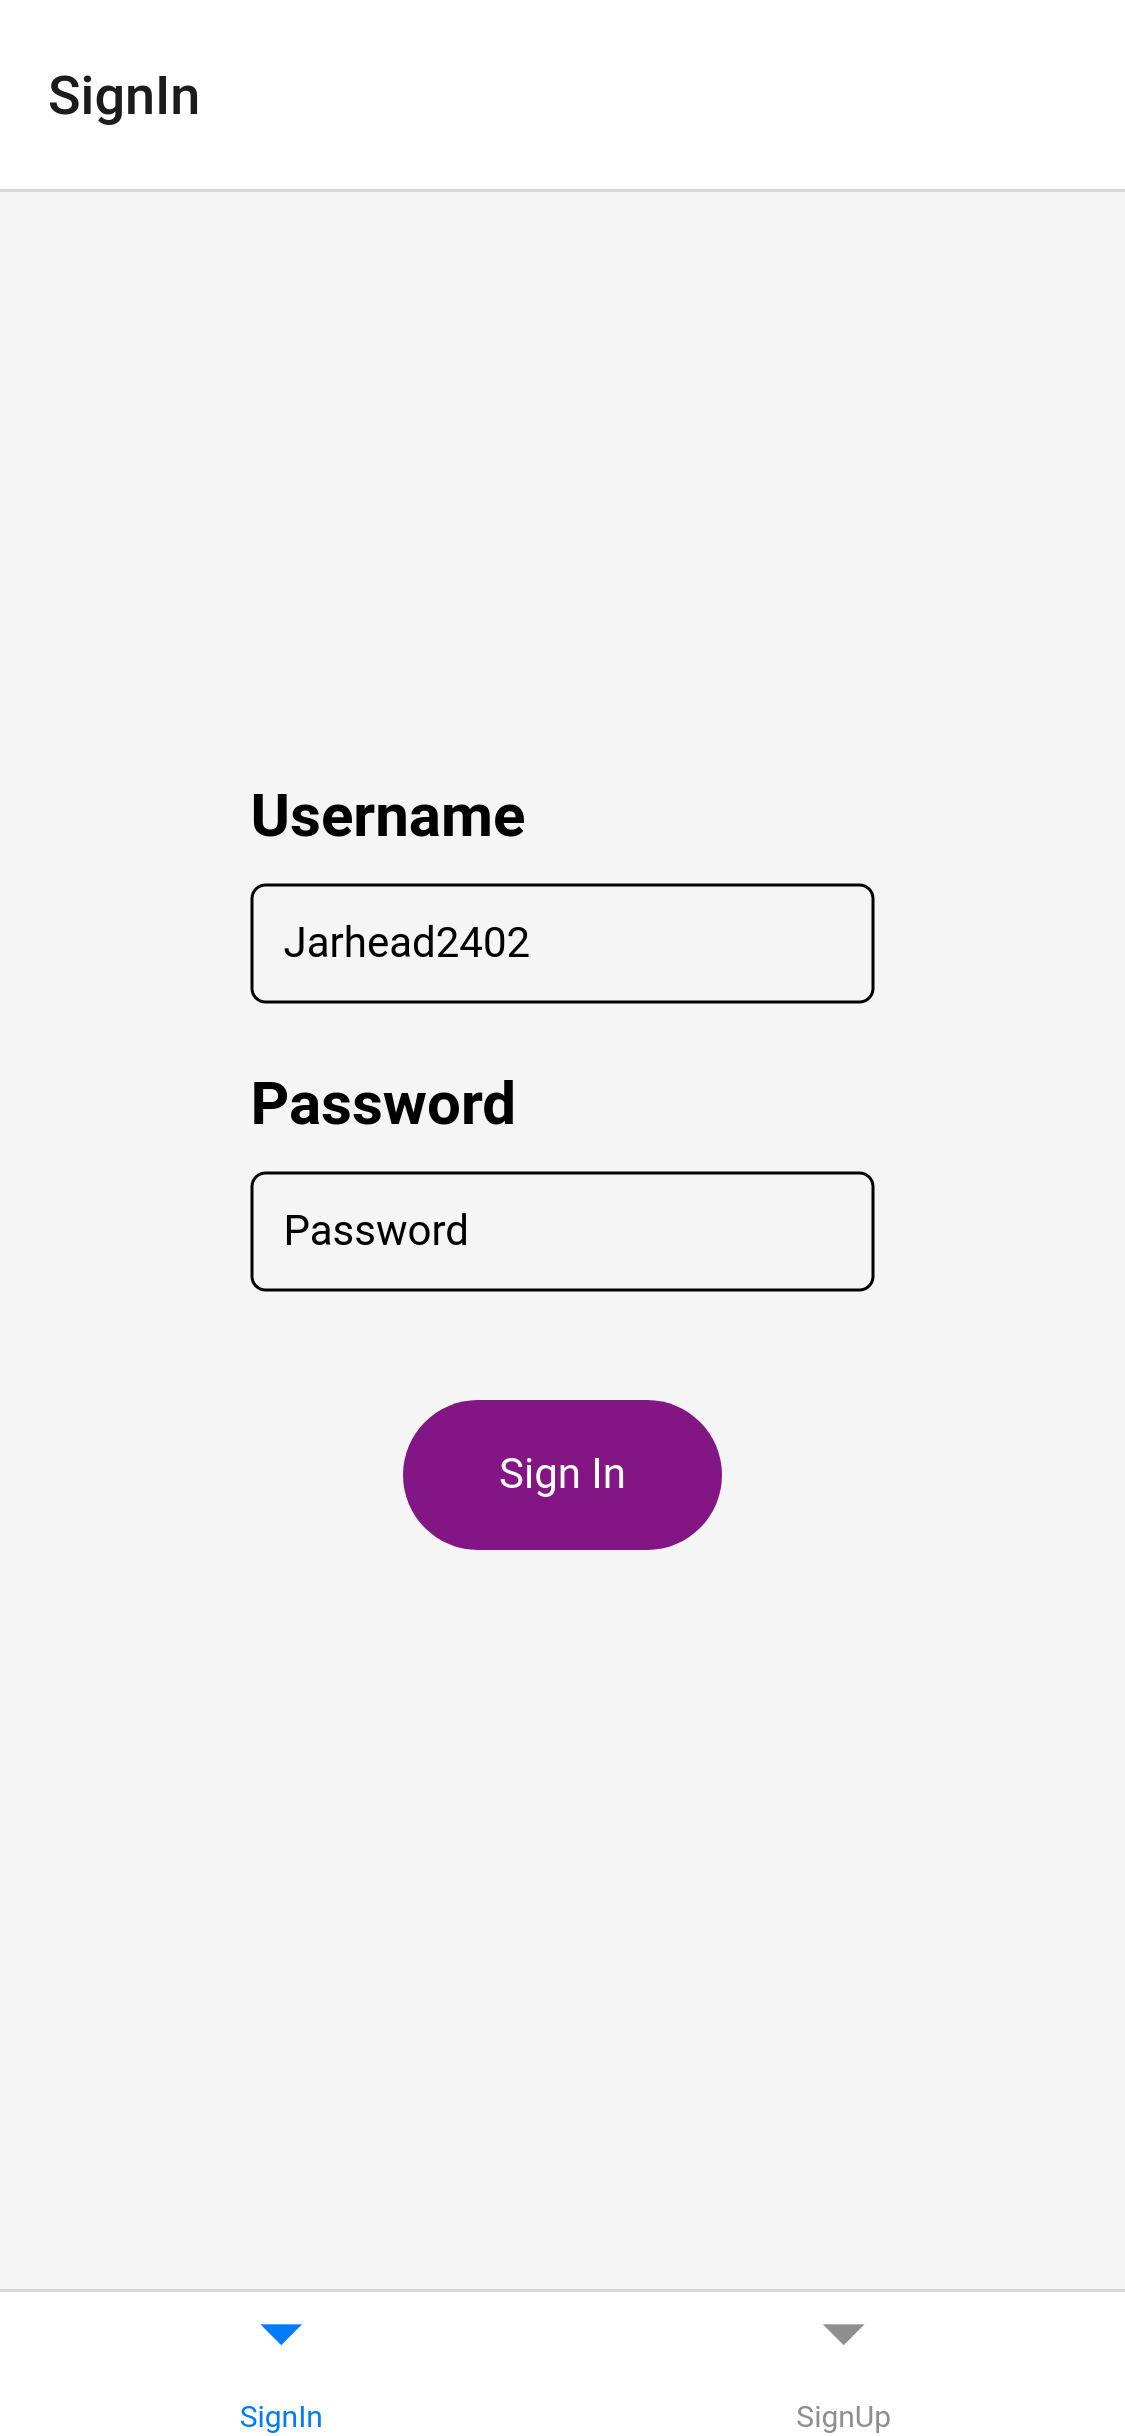
\includegraphics[width=0.45\textwidth]{images/signIn}
%            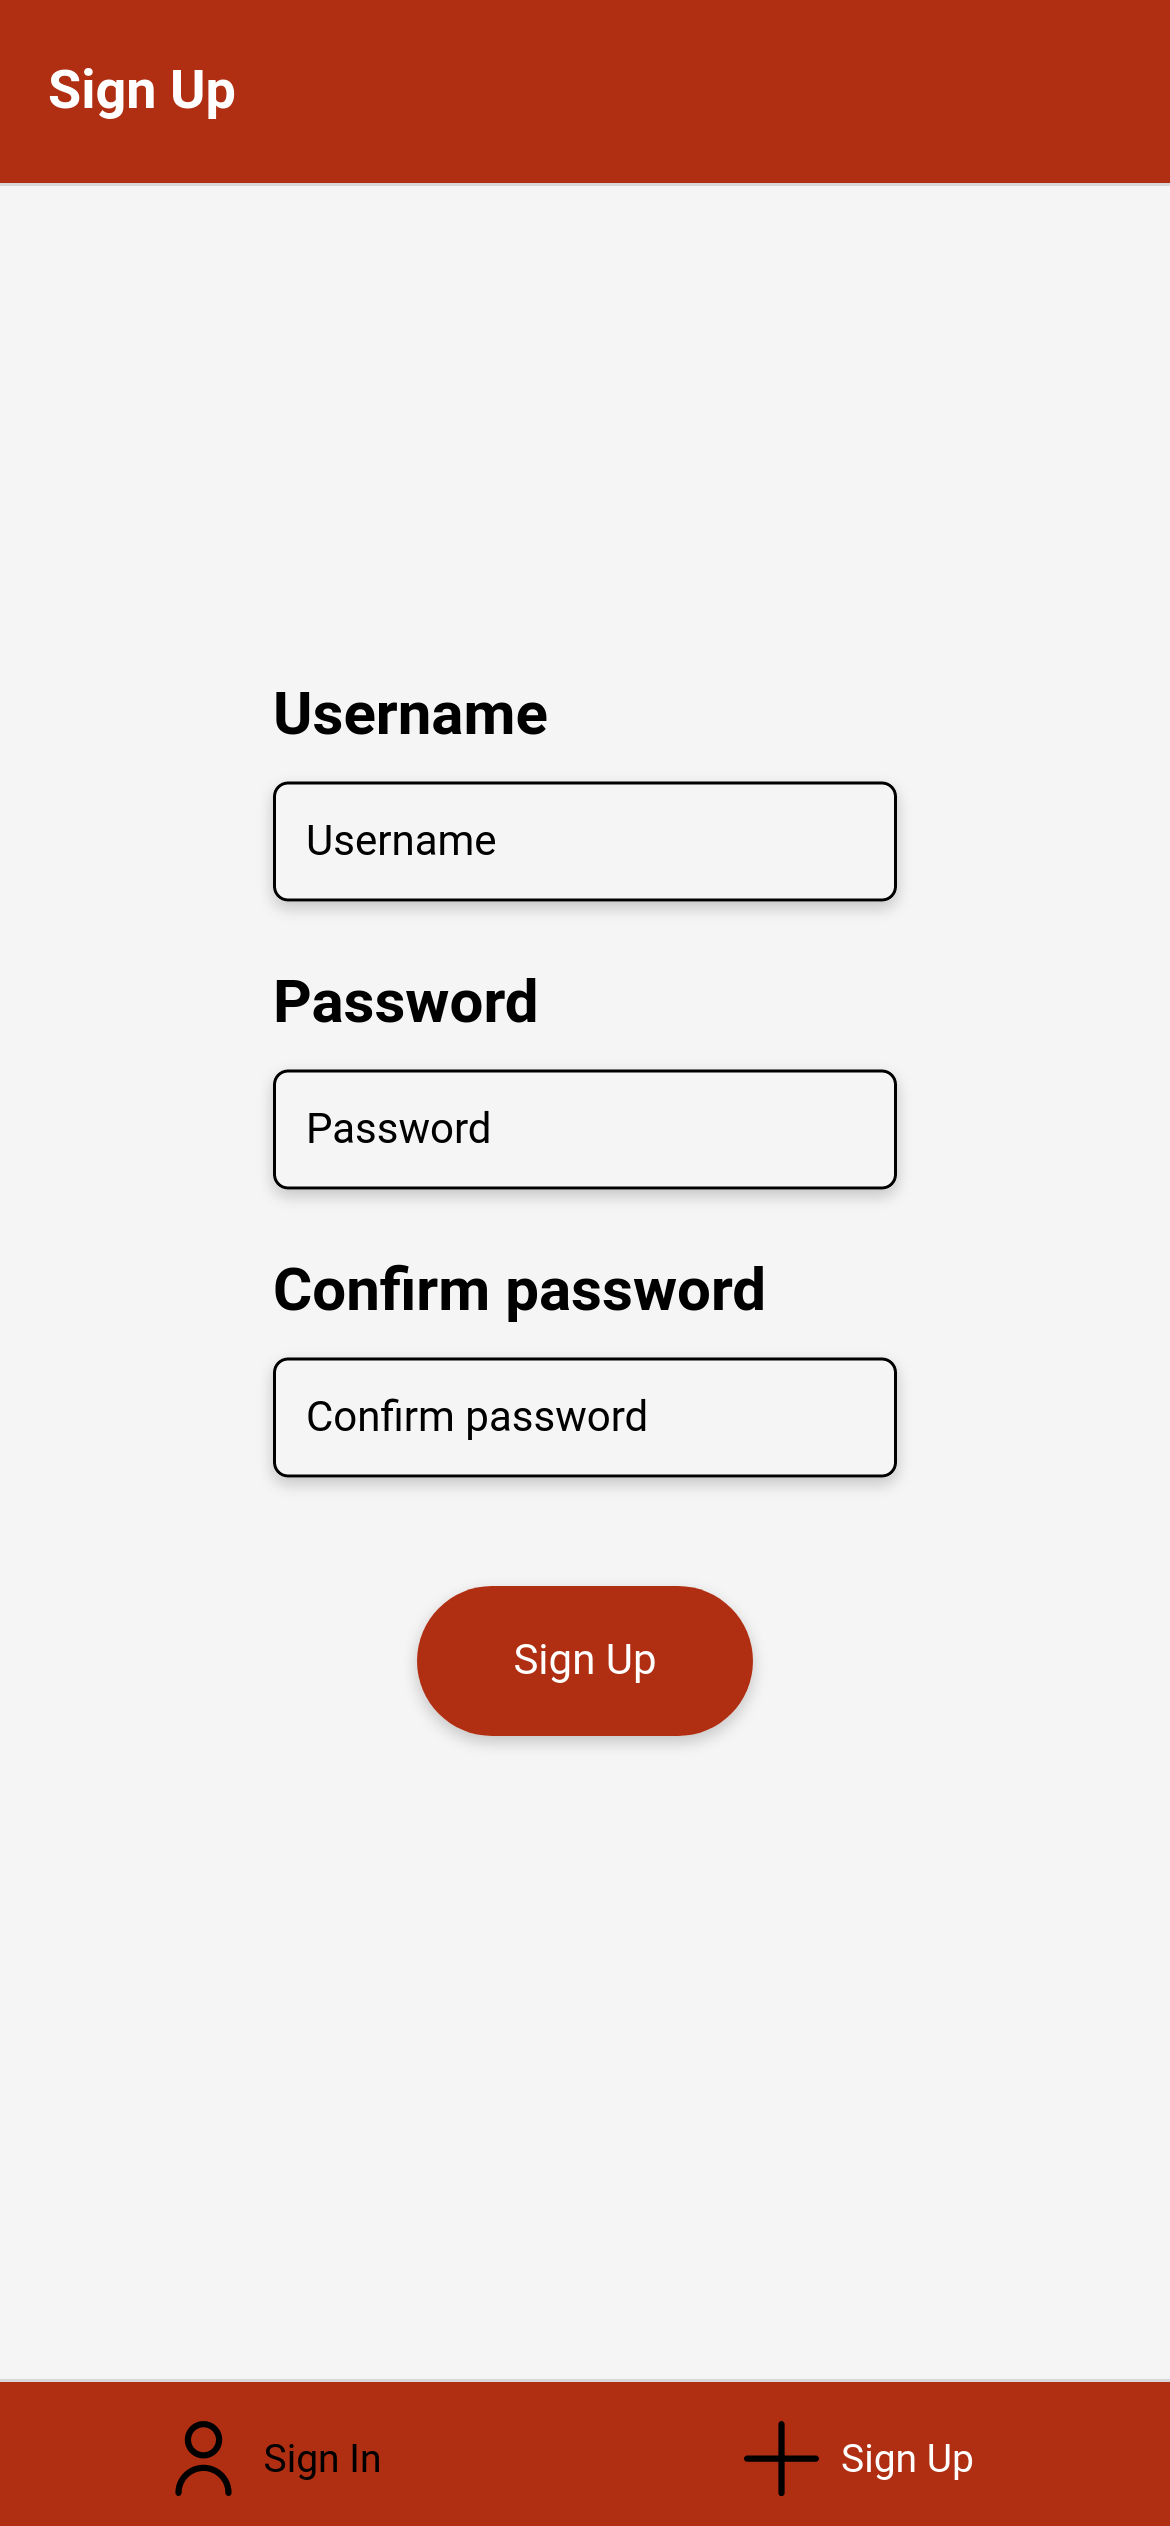
\includegraphics[width=0.45\textwidth]{images/signUp}
%            \caption{Ecran de connexion et d'inscription}
%            \label{fig:connexion}
%        \end{figure}
        % Afficher les 2 écrans de connexion et d'inscription coté à coté sur la même dans 2 figures différentes
        \begin{minipage}[t]{0.45\textwidth}
            \begin{figure}[H]
                \centering
                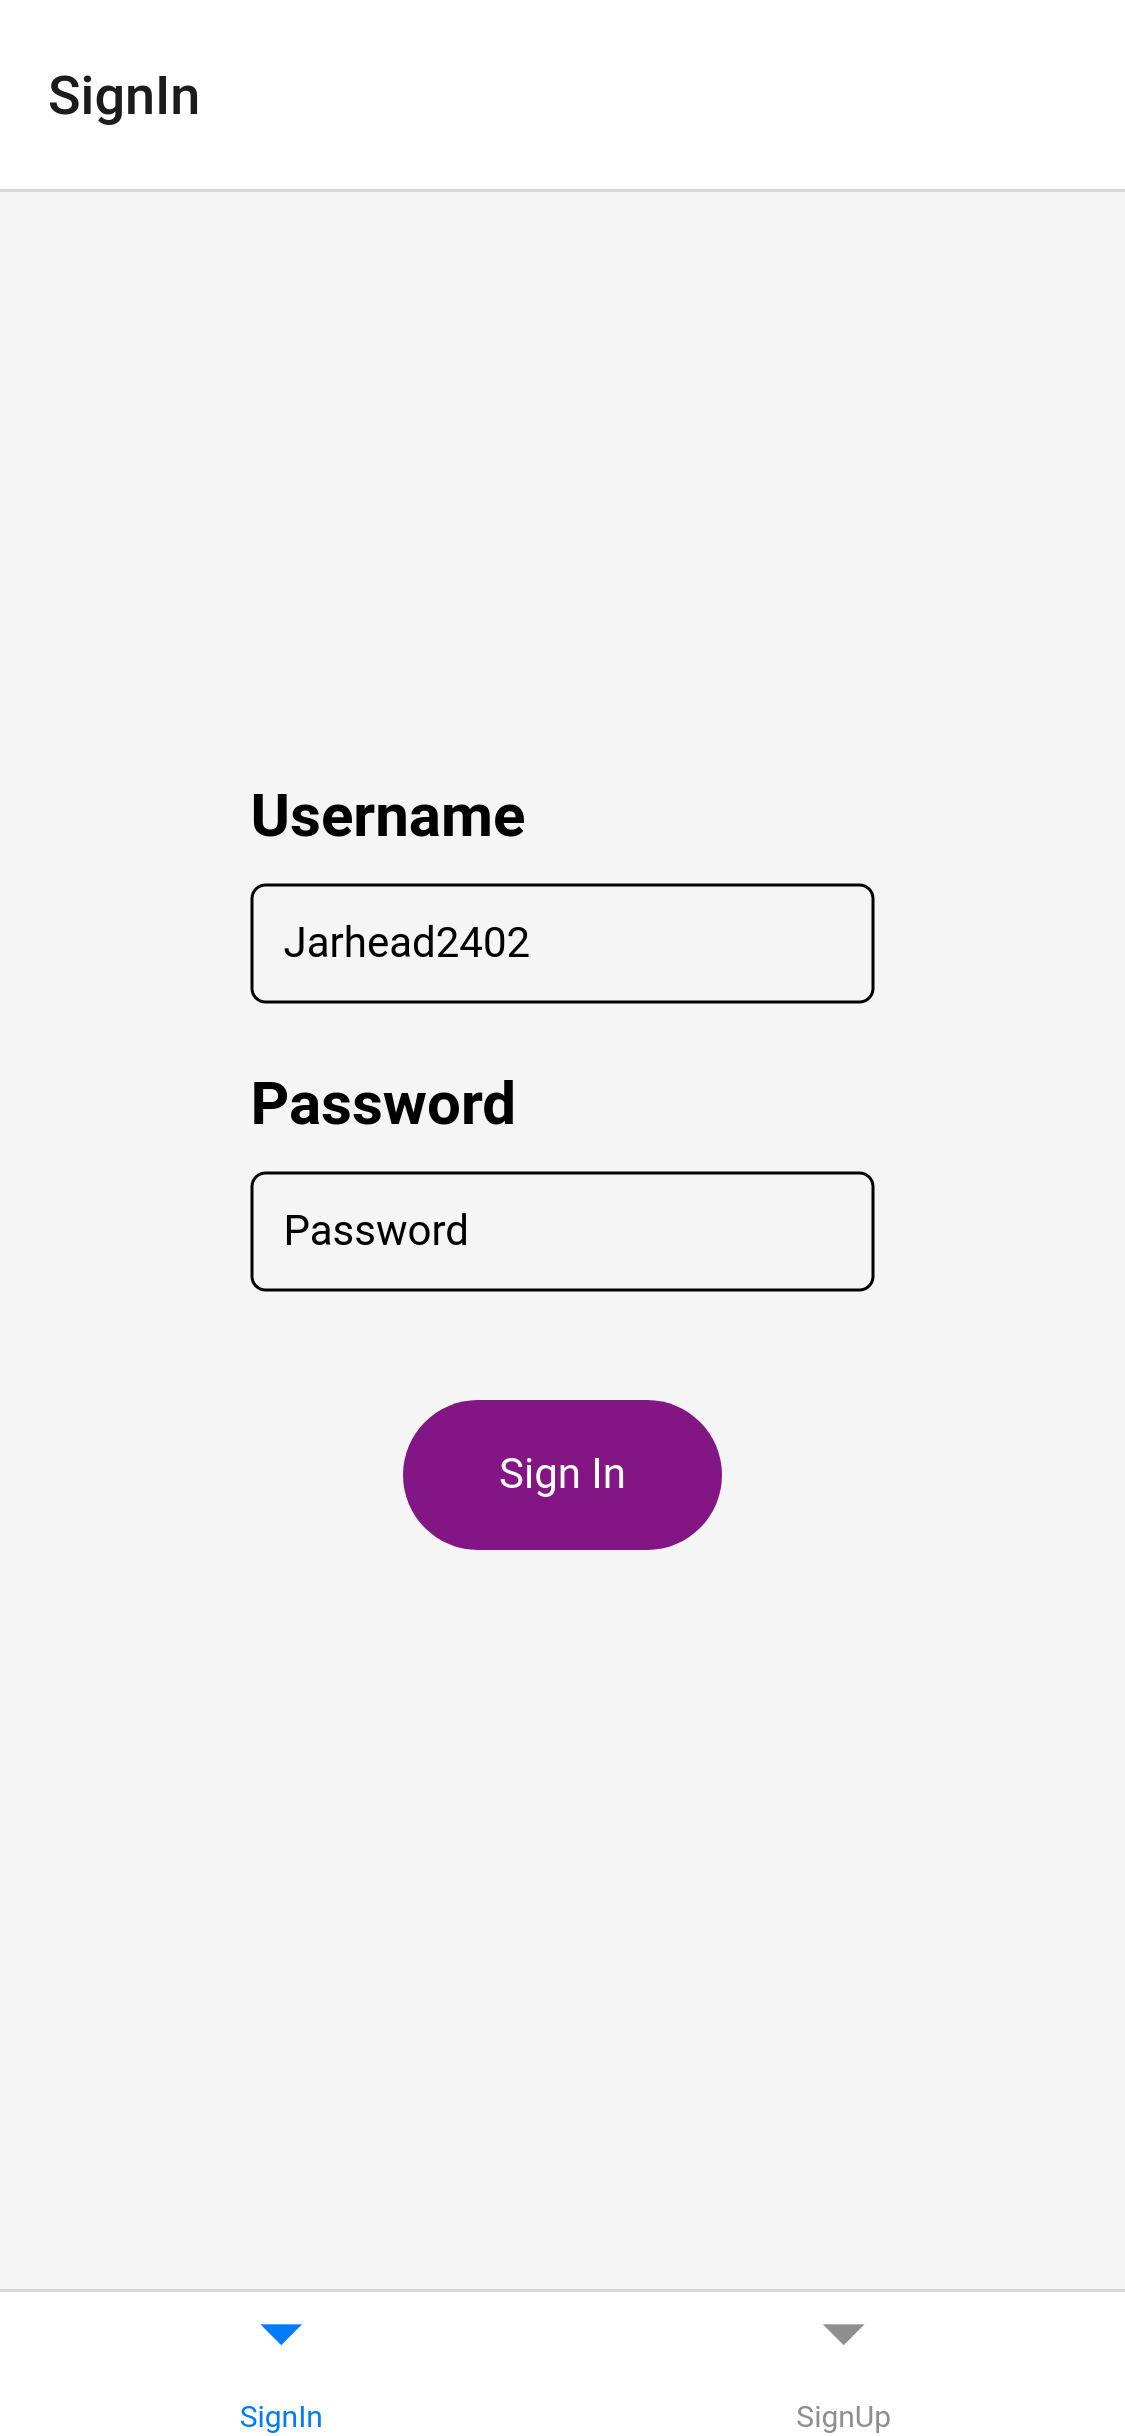
\includegraphics[scale=0.2]{images/signIn}
                \caption{Ecran de connexion}
                \label{fig:connexion}
            \end{figure}
        \end{minipage}
        \hspace{0.5cm}
        \begin{minipage}[t]{0.45\textwidth}
            \begin{figure}[H]
                \centering
                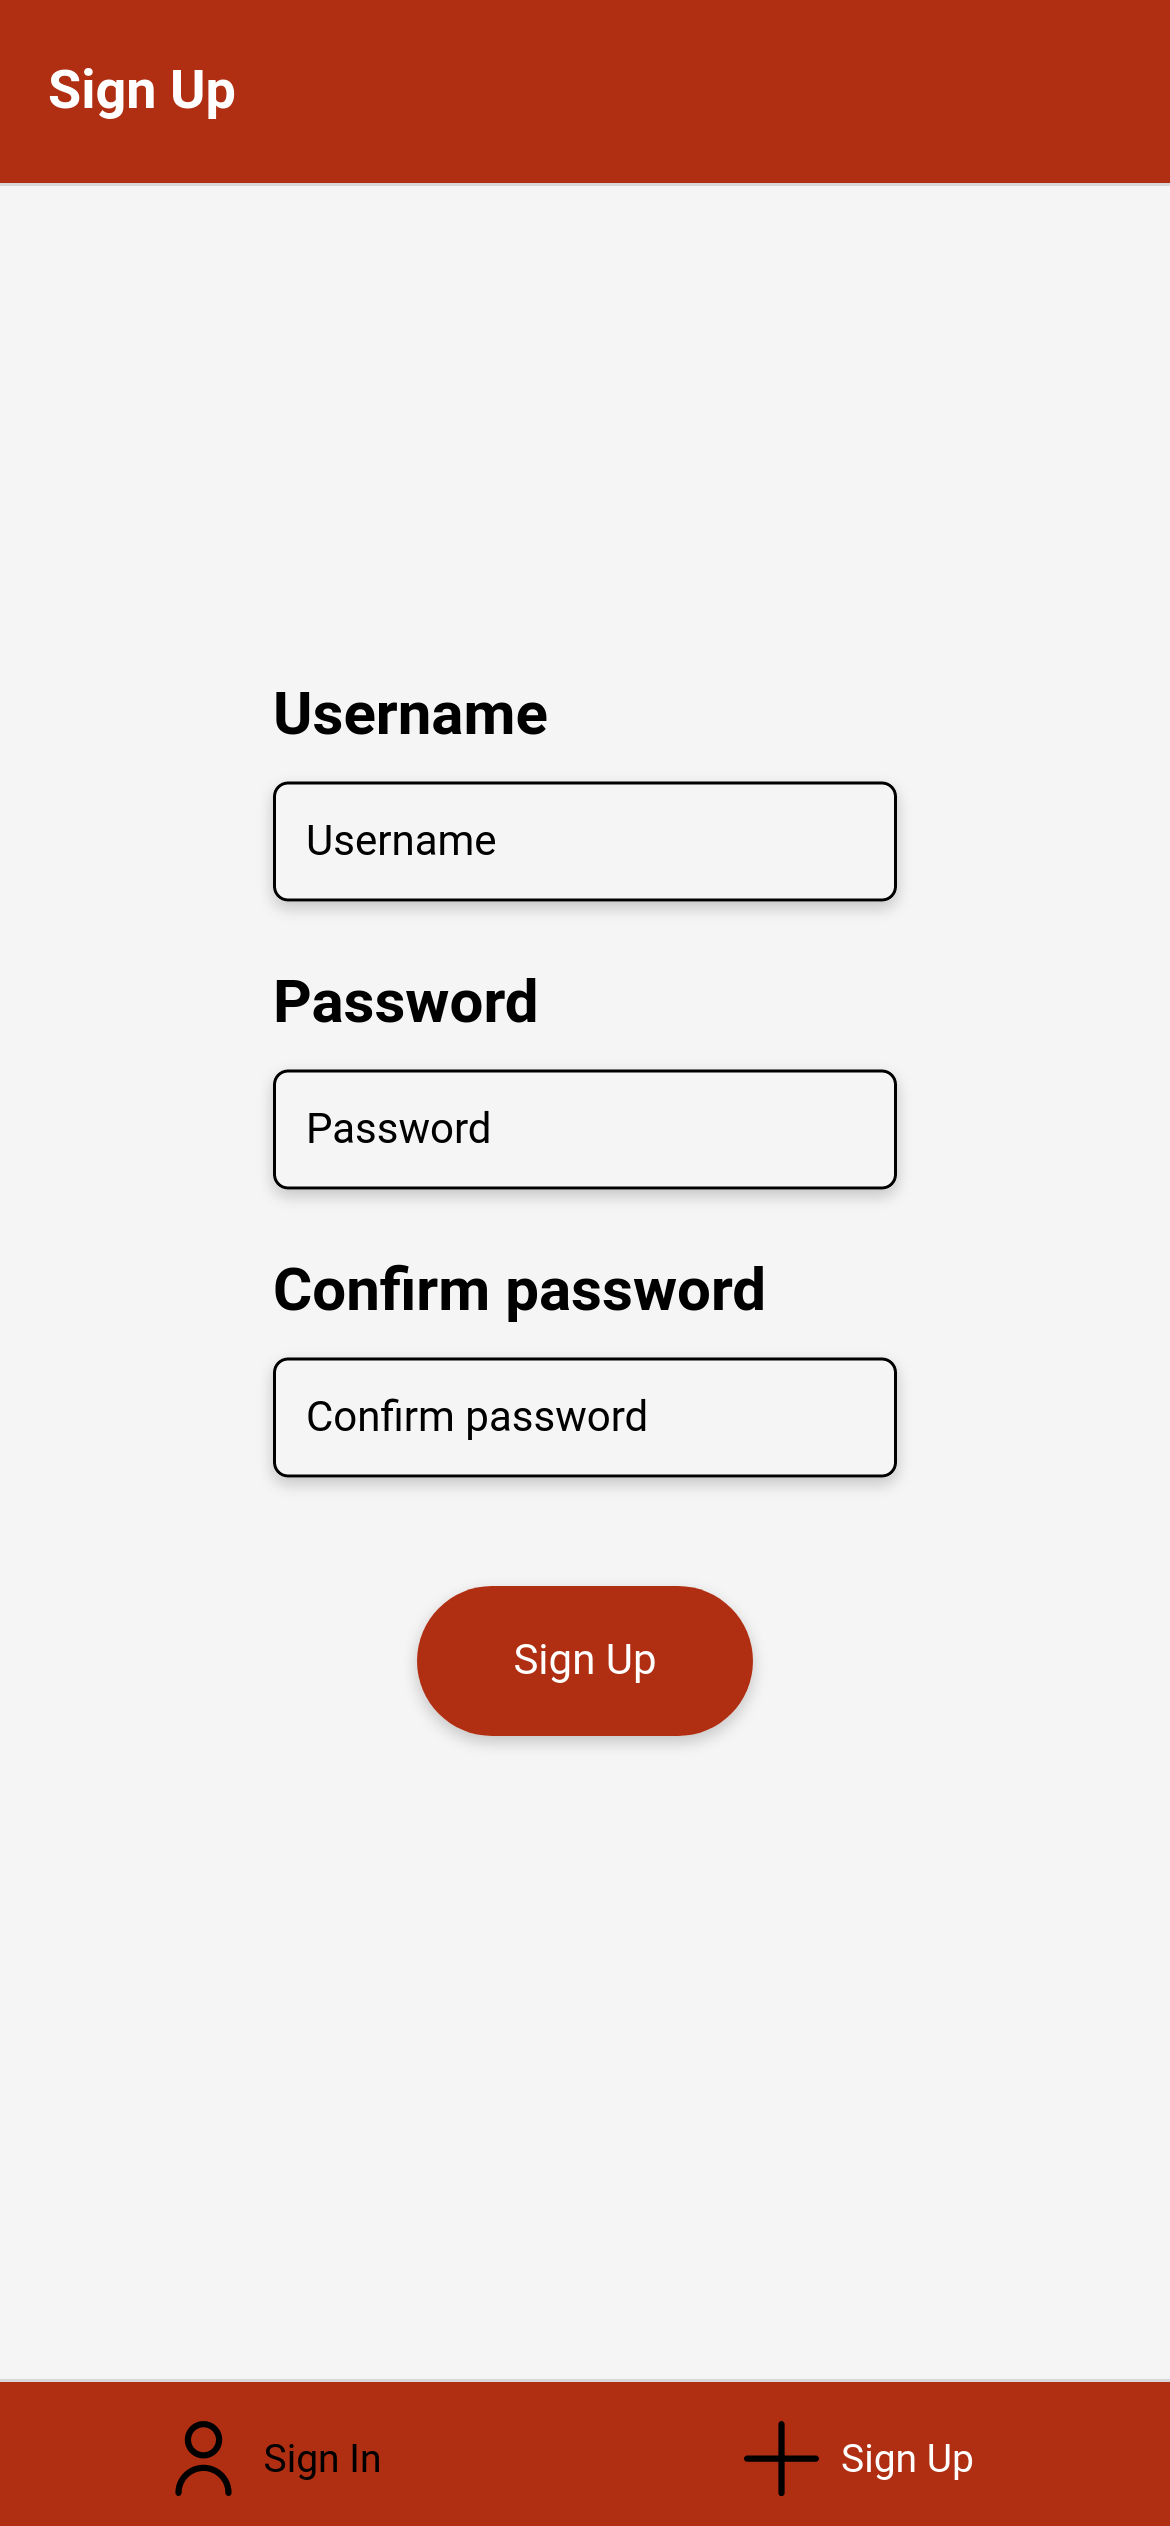
\includegraphics[scale=0.2]{images/signUp}
                \caption{Ecran d'inscription}
                \label{fig:inscription}
            \end{figure}
        \end{minipage}
        \\

        Un utilisateur qui souhaite utiliser l'application doit donc se créer un compte en renseignant son nom d'utilisateur,
        et son mot de passe\footnote{Le mot de passe doit être robuste, c'est à dire qu'il doit contenir au moins 8 caractères, dont au moins
        une lettre majuscule, une lettre minuscule, un chiffre. Cela permet de garantir la sécurité du compte de l'utilisateur
        dans le cas où celui-ci est piraté. De plus il faudrait dans une version ultérieure de l'application, hasher le mot de passe de l'utilisateur avant
        de le stocker dans la base de données}
        Une fois le compte créé, l'utilisateur peut se connecter à son compte en renseignant ces mêmes
        informations et accéder à ses tâches.

        \subsubsection{Manipulation des tâches}\label{subsubsec:manipulation-des-taches}
        Une fois connecté à son compte, l'utilisateur peut accéder à ses tâches. Il peut alors créer une nouvelle tâche,
        modifier le statut d'une tâche, ou encore supprimer une tâche. Dans la version actuelle de l'application, le statut
        d'une tâche se limite à : \textbf{todo}\footnote{La tâche n'a pas encore été effectuée}, \textbf{done}\footnote{La tâche a été effectuée}.

        % Afficher l'écran de gestion des tâches
        \begin{figure}[H]
            \centering
            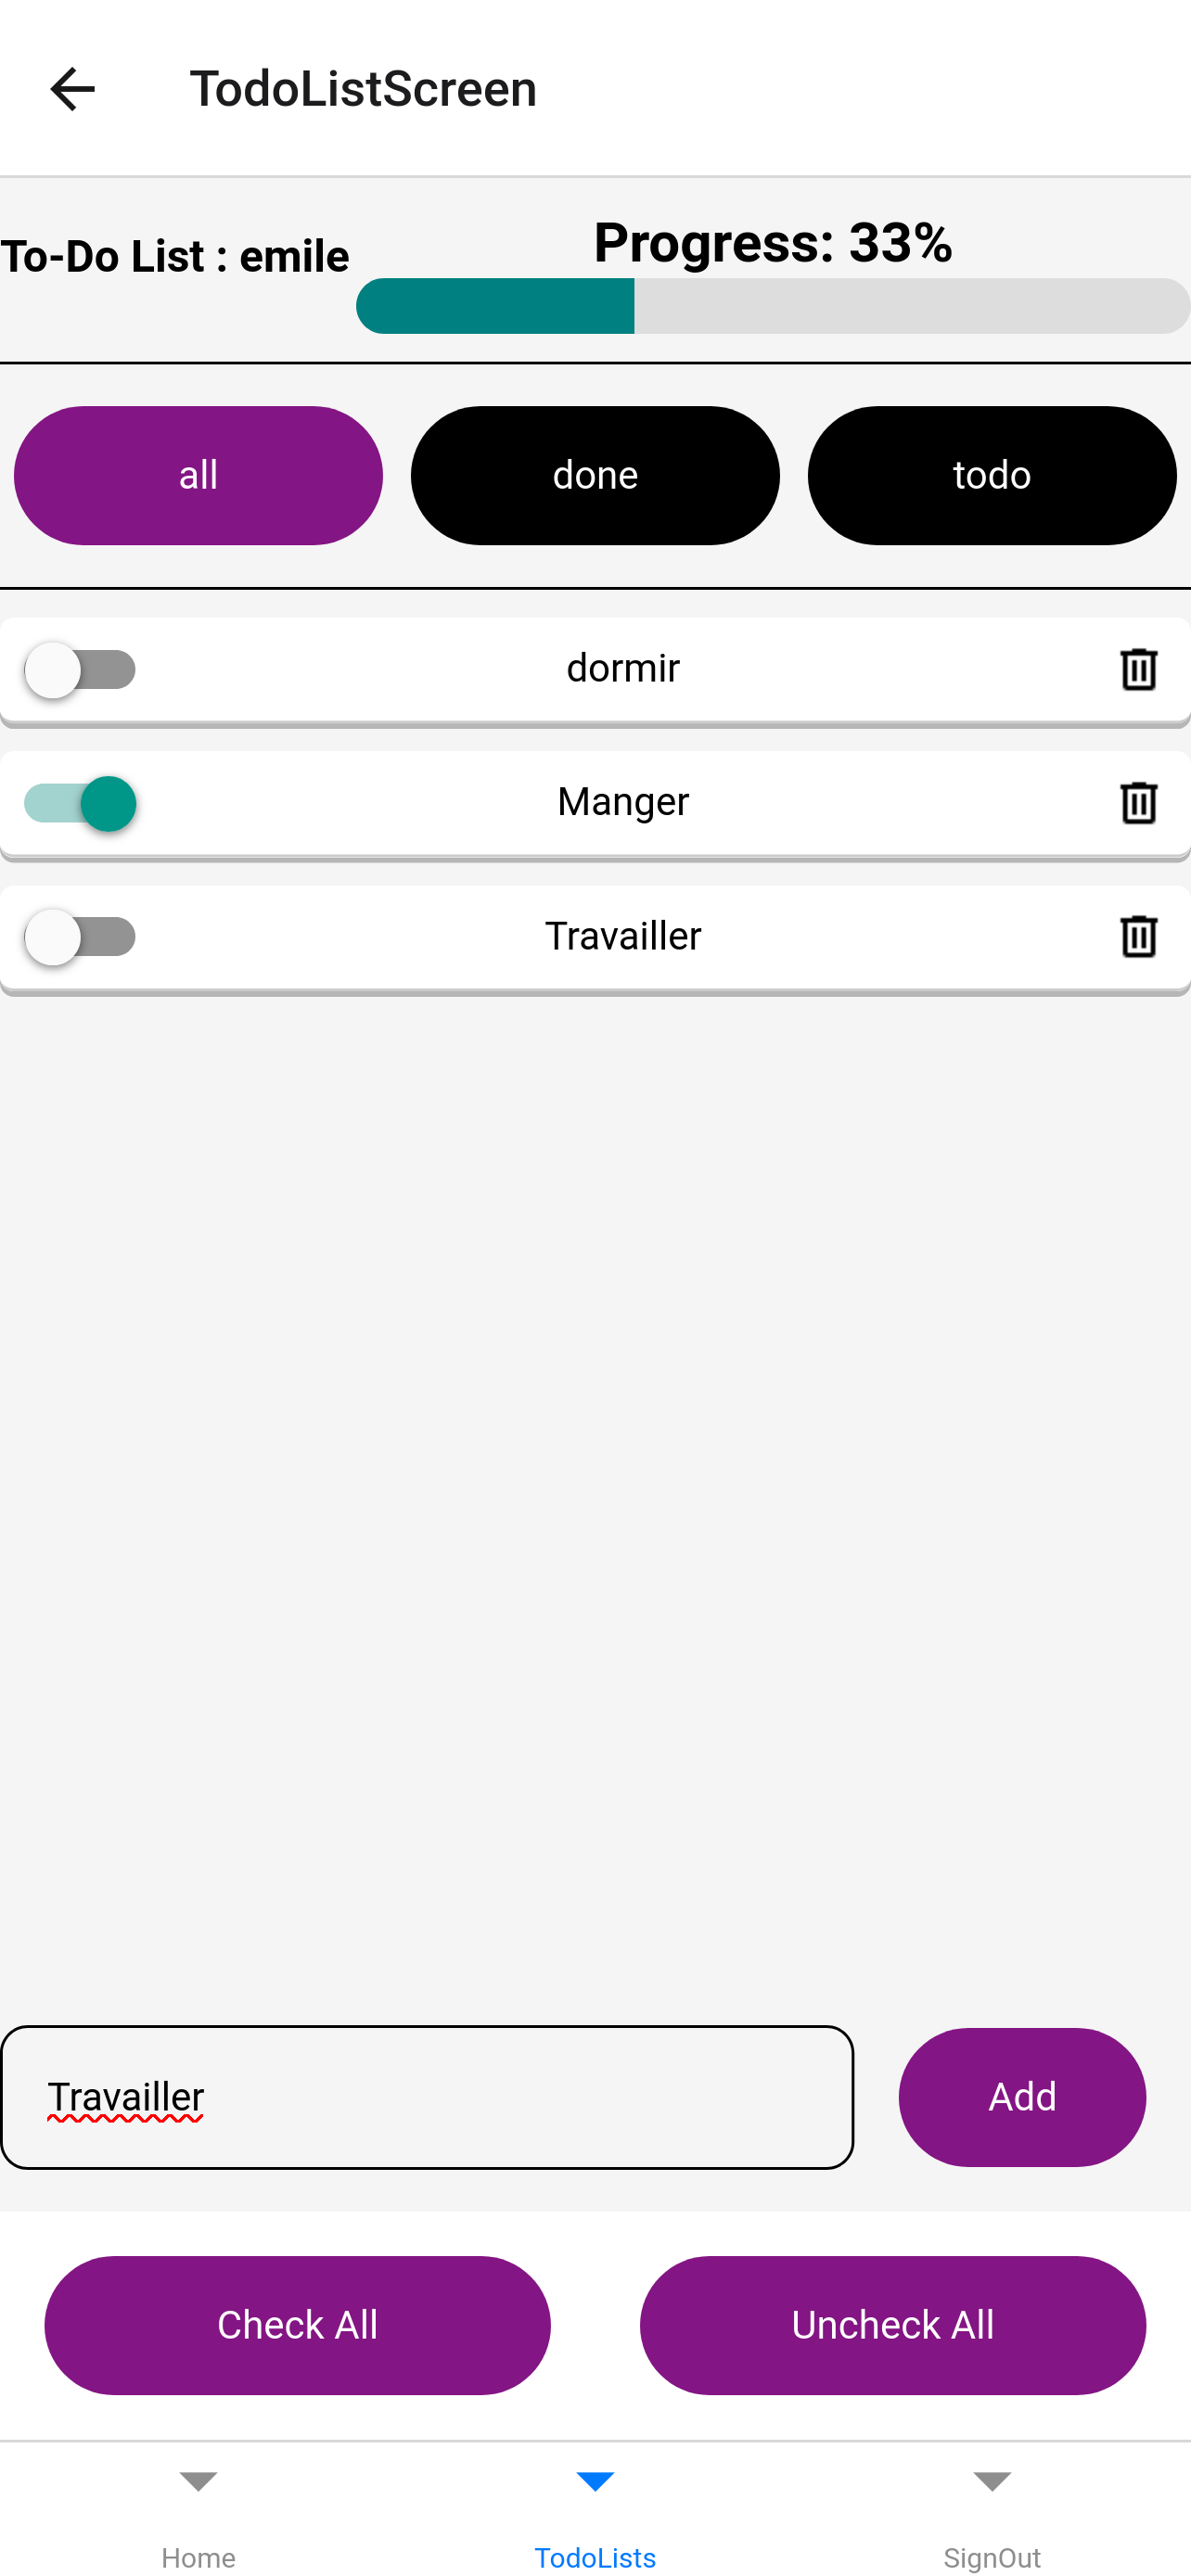
\includegraphics[scale=0.2]{images/tasks}
            \caption{Ecran de gestion des tâches}
            \label{fig:gestion-taches}
        \end{figure}

        Comme on peut le voir sur la figure \ref{fig:gestion-taches}, l'utilisateur peut créer une nouvelle tâche en
        remplissant le champ de texte en dessous de l'écran et en cliquant sur le bouton \textbf{Add}. Le choix
        a été fait de ne pas laisser la possibilité à l'utilisateur de créer une tâche vide. Cela permet de garantir
        que l'utilisateur ne crée pas de tâche sans contenu qui sont souvent inutiles et qui pollueront la liste des tâches.\\
        Le changement de statut d'une tâche se fait en cliquant sur le bouton \textbf{switch} à côté de la tâche et la suppression
        d'une tâche se fait en cliquant sur l'icône \textbf{trash} à côté de la tâche\footnote{La suppression d'une tâche est définitive et sans possibilité de récupération}\\

        Toutefois, il faut noter que l'utilisateur peut filtrer les tâches en fonction de leur statut. Il peut ainsi
        afficher uniquement les tâches qui sont à faire ou celles qui ont déjà été effectuées et donc mieux gérer ses tâches.\\
        Une possibilité lui a été aussi donnée de rendre toutes ses tâches à faire en cliquant sur le bouton \textbf{Reset} ou
        de les marquer toutes comme effectuées en cliquant sur le bouton \textbf{Done}.\\

        \subsection[Bonus]{Fonctionnalités avancées}\label{subsec:fonctionnalites-avancees}
        Ces fonctionnalités sont des fonctionnalités qui ont été ajoutées à l'application pour améliorer l'expérience utilisateur.
        Certaines d'entre elles sont uniquement des questions de confort, style ou de design, d'autres par contre sont
        des fonctionnalités qui permettent d'augmenter la productivité de l'utilisateur et emmènent l'application vers
        une autre dimension d'utilisation.\\

        \subsubsection{Gestions des listes de tâches}\label{subsubsec:gestion-des-listes-de-taches}
        Dans une application de gestion de tâches, on peut se retrouver avec une liste de tâches très longue et
        très difficile à gérer. De plus, il peut être intéressant de pouvoir regrouper des tâches en fonction de leur
        thème ou de leur catégorie.\\
        C'est pourquoi, EasyTasks permet à l'utilisateur de créer des listes de tâches. Il peut ainsi créer une liste
        de tâches pour ses tâches professionnelles, une autre pour ses tâches personnelles, une autre pour ses tâches
        de sport, etc.\\
        Cette fonctionnalité est un gros gain de productivité pour l'utilisateur, car il peut ainsi mieux organiser ses tâches
        à sa convenance.

        % Afficher l'écran de gestion des listes de tâches
        \begin{figure}[H]
            \centering
            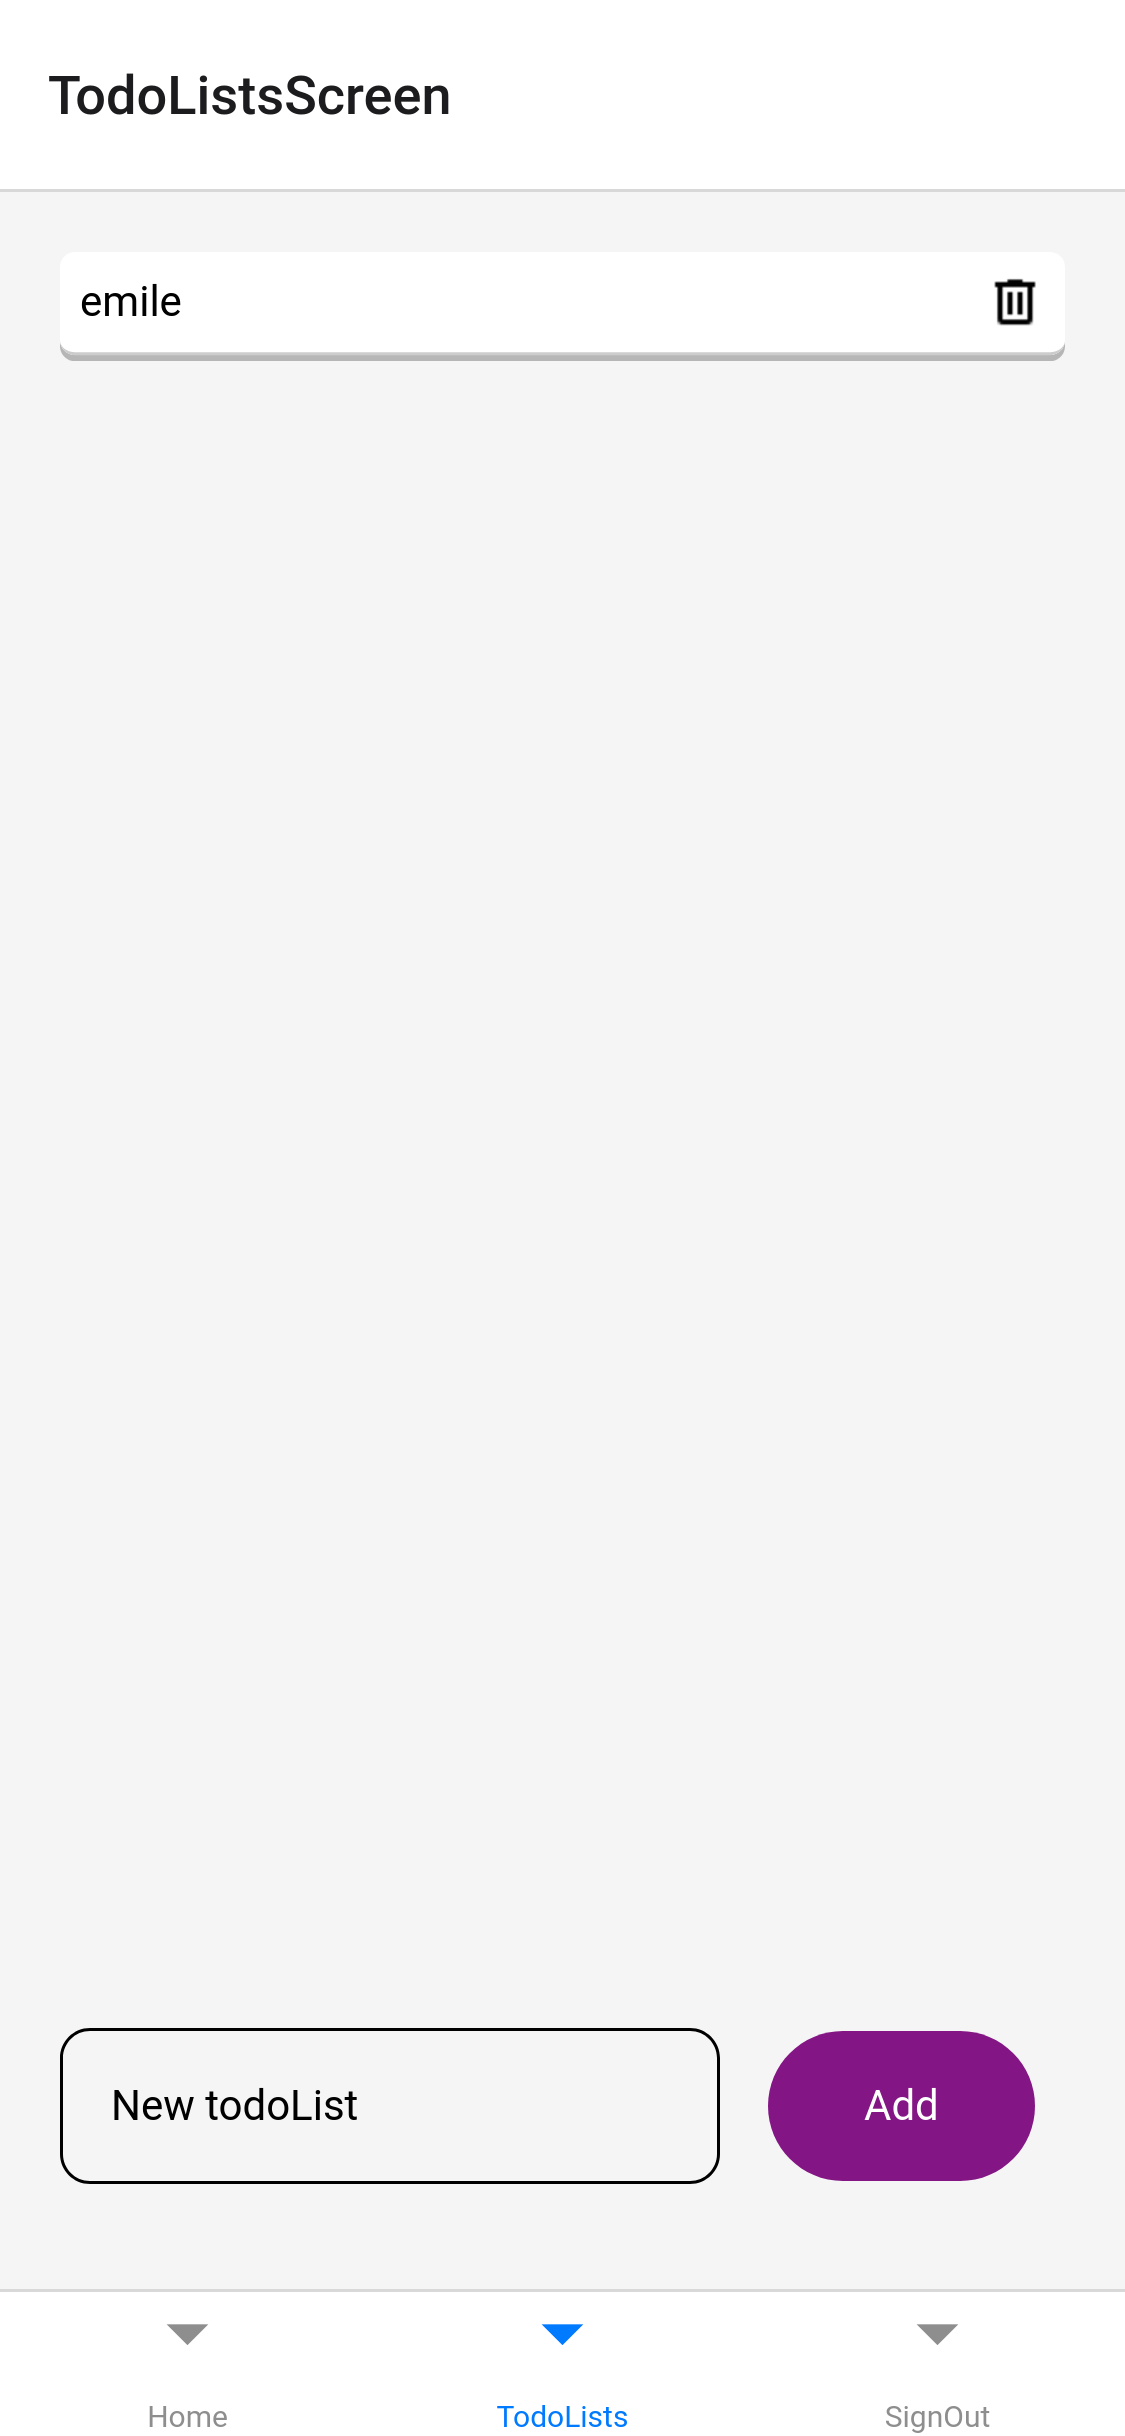
\includegraphics[scale=0.15]{images/taskList}
            \caption{Ecran de gestion des listes de tâches}
            \label{fig:gestion-listes}
        \end{figure}

        L'utilisateur peut créer une nouvelle liste de tâches voir la figure \ref{fig:gestion-listes} en remplissant
        le champ de texte et en cliquant sur le bouton \textbf{Add}.\\ Chaque item de la liste représente une liste de tâches
        et est cliquable. En cliquant sur un item, l'utilisateur est redirigé vers l'écran de gestion des tâches(voir figure \ref{fig:gestion-taches})
        et peut alors gérer les tâches de cette liste.\\
        La possibilité a été donnée à l'utilisateur de supprimer une liste de tâches en cliquant sur l'icône \textbf{trash}.
        Mais aussi de renommer une liste de tâches en maintenant pendant quelques secondes l'item de la liste.

        \subsubsection{Gestion des utilisateurs}\label{subsubsec:gestion-des-utilisateurs}
        Etant donné que chaque utilisateur a son propre compte, il est important de pouvoir non seulement donner la possibilité
        à l'utilisateur de personnaliser son compte, mais aussi à un administrateur de pouvoir gérer les comptes des utilisateurs
        dans le cas où un utilisateur ne respecte pas les règles de l'application. Bien que la gestion des utilisateurs
        puisse être opérée directement dans la base de données, il est plus pratique de pouvoir le faire directement dans l'application.
        Cela a d'énormes avantages:
        \begin{itemize}
            \item L'administrateur n'a pas besoin de connaître les manipulations à faire dans la base de données pour pouvoir gérer les comptes des utilisateurs.
            \item L'administrateur peut gérer les comptes des utilisateurs sans avoir à se connecter à la base de données\footnote{Toutefois, il doit se connecter à l'application pour pouvoir gérer les comptes des utilisateurs}.
            \item Le client pour qui l'application a été développée n'a pas besoin d'être un expert en base de données ou informatique pour pouvoir gérer les comptes des utilisateurs.
            \item Une assistance constante du développeur (ou d'un autre développeur) n'est pas nécessaire durant toute la durée de vie de l'application.
        \end{itemize}
        \vspace{0.5cm}
        % Afficher l'écran de gestion des utilisateurs pour un utilisateur normal et un administrateur
        \begin{minipage}[t]{0.45\textwidth}
            \centering
            \begin{figure}[H]
                \centering
                \includegraphics[widht=0.5\textwidth]{images/user}
                \caption{Profil utilisateur}
                \label{fig:gestion-utilisateurs-normal}
            \end{figure}
        \end{minipage}
        \hspace{0.5cm}
        \begin{minipage}[t]{0.45\textwidth}
            \centering
            \begin{figure}[H]
                \centering
                \includegraphics[widht=0.5\textwidth]{images/admin}
                \caption{Profil administrateur}
                \label{fig:gestion-utilisateurs-admin}
            \end{figure}
        \end{minipage}
        \vspace{0.5cm}

        L'écran de gestion des utilisateurs est accessible depuis tout écran de l'application en cliquant sur le bouton \textbf{Profile}.
        Depuis cet écran, tout utilisateur peut modifier ses informations personnelles\footnote{Dans cette version, seul le nom de l'utilisateur peut être modifié.} ou bien se déconnecter de l'application.
        L'administrateur peut aussi gérer les comptes des utilisateurs en cliquant sur le bouton \textbf{Liste des utilisateurs}. De ce fait, l'option
        \textbf{Liste des utilisateurs}.est visible uniquement pour les administrateurs.\\
        L'écran de gestion des utilisateurs permet à l'administrateur de pouvoir supprimer un compte d'utilisateur,
        de pouvoir modifier le rôle d'un utilisateur (administrateur ou utilisateur normal) \footnote{La modification du mot de passe d'un utilisateur est interdite pour des raisons de sécurité.\\
        La création d'un nouveau compte utilisateur passe par l'inscription de l'utilisateur(voir section\ref{subsubsec:authentification}).}.
        Pour toutes ces actions à part la suppression d'un compte utilisateur, l'administrateur doit cliquer sur l'item de l'utilisateur
        qu'il souhaite modifier pour avoir plus d'informations sur cet utilisateur.\\

        Bien qu'il a été demandé d'implémenter 2 bonus au choix, nous nous sommes permis d'implémenter d'autres fonctionnalités:
        \begin{itemize}
            \item \textbf{Une barre de progression}: Cette barre de progression permet à l'utilisateur de voir l'avancement de ses tâches.
            \item \textbf{Une interface utilisateur soignée}: L'interface utilisateur a été soignée pour que l'utilisateur puisse avoir une expérience utilisateur agréable.
        \end{itemize}
        Ils ont été implémentés pour améliorer l'expérience utilisateur et pour donner une meilleure image de l'application.

        \section{Détails techniques}\label{sec:details-techniques}

        \subsection{Architecture}\label{subsec:architecture}
        L'application a été développée en utilisant le framework React Native. React Native est un framework qui permet de développer des applications multiplateformes.
        Il permet de développer pouvant être exécutées dans différents environnements sans avoir à réécrire le code\footnote{Le code est écrit une seule fois et peut être exécuté sur plusieurs plateformes.}.
        React Native est basée sur le framework React qui est un framework JavaScript. React Native utilise le langage JavaScript pour le développement de l'application.\\
        Ainsi le code de l'application inclut les composants et la logique métier de l'application.\\

        Au niveau le plus haut de l'architecture, l'application est composée d'un seul composant qui est le composant principal de l'application(\textbf{App.js}).
        Ce composant est le point d'entrée de l'application. Il est chargé de charger les autres composants de l'application.\\
        En dessous du composant principal, il y a le composant de navigation. Ce composant est chargé de gérer la navigation entre les différents écrans de l'application.
        EasyTask utilise cinq (5) écrans principaux dont trois ne sont accessibles que pour les utilisateurs connectés. Chaque écrans charge
        les composants dont il a besoin pour fonctionner.\\

        Ainsi, l'architecture de l'application est hierarchique. Chaque composant est chargé de gérer une partie de l'application. De
        ce fait un composant parent contient et affiche ses composants enfants.\\

        \subsection{Composants réutilisables}\label{subsec:composants-reutilisables}
        Durant le développement de l'application, nous avons remarqué que certains composants étaient réutilisables dans plusieurs
        écrans. En effet, des composants comme les boutons, les champs de texte, les listes(taches, utilisateurs, listes de tâches)...
        étaient utilisés dans plusieurs écrans. Pour éviter de répéter le code de ces composants, nous avons décidé de les
        encapsuler dans des composants personnalisés. Les encapsuler étaient une bonne idée car cela permettait de réduire le code
        et de le rendre plus lisible, mais aussi d'avoir une certaine cohérence et une certaine uniformité dans l'application.

        \subsubsection{Boutons}\label{subsubsec:boutons}
        Les boutons sont des composants réutilisables dans plusieurs écrans. Ils sont utilisés pour les actions de l'utilisateur
        comme : se connecter, se déconnecter, créer une tâche, modifier une tâche, supprimer une tâche et bien d'autres.
        Pour éviter de répéter le code/style des boutons, nous avons décidé de les encapsuler dans un composant propre à l'application.
        Ce composant est appelé \textbf{ButtonComponent} et il est défini dans le fichier \textbf{buttonComponent.js}.  Leur
        fonctionnement et leur utilisation ne sont pas si différents de ceux des boutons de base de React Native.\\
        % Afficher un exemple de bouton
        \begin{figure}[H]
            \centering
            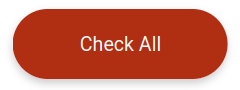
\includegraphics[width=0.45\textwidth]{images/button}
            \caption{Exemple de bouton}
            \label{fig:button}
        \end{figure}

        La particularité de ce composant est qu'il peut être stylisé en fonction de l'écran dans lequel il est utilisé avec
        beaucoup plus de facilité et de liberté que les boutons de base de React Native. Par défaut, ce button
        est arrondi sur les bords et il a une couleur de fond marron.

        \subsubsection{Champs de texte}\label{subsubsec:champs-de-texte}
        On réutilise les champs de texte à chaque fois qu'on veut demander à l'utilisateur de saisir une information.
        Ainsi pour ne pas se répéter dans le style que l'on donne à ces champs de texte dans notre application, nous avons
        décidé de les encapsuler dans un composant propre à l'application. Ce composant est appelé \textbf{Field}
        et il est défini dans le fichier \textbf{field.js}.\\
        % Afficher un exemple de champ de texte
        \begin{figure}[H]
            \centering
            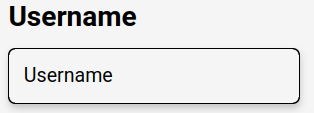
\includegraphics[width=0.45\textwidth]{images/field}
            \caption{Exemple de champ de texte}
            \label{fig:field}
        \end{figure}
        Il n'y a pas de différence notable entre les champs de texte de base de React Native et ce composant. La particularité
        se résume à l'aspect visuel du champ de texte qui possède un style plus soigné que celui des champs de texte de base de React Native.
        Un petit effet d'arrondir sur les bords et un effet de flottaison sont ajoutés au champ de texte pour améliorer son aspect visuel.

        \subsubsection{Items}\label{subsubsec:items}
        Souvent nous avons besoin d'afficher des informations dans une liste. Par exemple, dans la liste des tâches, nous avons besoin
        d'afficher le nom de la tâche, dans la liste des utilisateurs, nous avons besoin d'afficher le nom de l'utilisateur, ainsi
        de suite. Ainsi, notre souhait étaient à partir du moment où nous avons besoin d'afficher des informations dans une liste,
        Les items de toutes les différentes listes devraient avoir un aspect assez commun. Et étant donné que le style de ces items
        ont été beaucoup travaillé, nous avons décidé de les encapsuler dans un composant propre à l'application. Ce composant est appelé
        \textbf{Item} et il est défini dans le fichier \textbf{Item.js}.\\
        % Afficher un exemple d'item
        \begin{figure}[H]
            \centering
            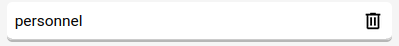
\includegraphics[width=0.45\textwidth]{images/item}
            \caption{Exemple d'item}
            \label{fig:item}
        \end{figure}

        % Décrire l'aspect visuel de l'item

        \subsubsection{Barre de progression}\label{subsubsec:barre-de-progression}
        Dans une application, nous avons souvent besoin de fournir à l'utilisateur une indication sur l'avancement globale
        d'une tâche, d'un processus, d'une opération, etc. Nous pourrions bien évidement décrire à l'utilisateur ces
        avancements en utilisant des mots, mais cela prendrait beaucoup de temps et de place. Mais aussi, cela serait moins
        parlant que de le lui montrer directement via des barres de progression accompagnées ou non de pourcentages.\\
        C'est dans cette optique que celle-ci a été développée. Elle est définie dans le fichier \textbf{progressBar.js}.
        % Afficher un exemple de barre de progression
        \begin{figure}[H]
            \centering
            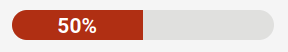
\includegraphics[width=0.45\textwidth]{images/progress-bar}
            \caption{Exemple de barre de progression}
            \label{fig:progress-bar}
        \end{figure}
        Cette barre de progression peut être utilisée dans n'importe quel écran de l'application. Elle est très flexible et
        elle peut être stylisée en fonction de l'écran dans lequel elle est utilisée. Elle peut aussi être utilisée avec ou sans
        pourcentage.\\


        % Interet de l'utilisation de composants réutilisables
        Le plus grand intérêt de l'utilisation de composants réutilisables est que cela nous permet de réduire le temps de développement
        de notre application. En effet, nous n'avons pas à répéter le code et le style de chaque composant à chaque fois que nous en avons besoin.
        Nous n'avons qu'à l'importer et à l'utiliser. De plus, cela nous permet de réduire la taille du code source de notre application. Le plus
        gros gain est celui relatif aux dépendances. En effet, beaucoup de ces composants ont pu déja être développés par d'autres
        développeurs et ils sont disponibles sur internet. Cependant, cela conduirait à une dépendance forte de notre application à des librairies
        externes. Le gros inconvénient d'utiliser des composants externes est que nous ne pouvons pas les modifier à notre guise et
        aussi à partir du moment où ces librairies ne sont plus maintenues, cela pourrait poser des problèmes à notre application.

        \section{Conclusion}\label{sec:conclusion}
        En conclusion, le développement de l'application EasyTask en react native a été une expérience enrichissante.
        Nous avons réussi à mettre en place les fonctionnalités de base de gestion de tâches et d'authentification des utilisateurs,
        ainsi que des fonctionnalités avancées de gestion des utilisateurs et des listes de tâches.\\

        Cependant, nous avons également rencontré des difficultés liées à la découverte de react native. Malgré cela,
        nous avons su surmonter ces obstacles grâce à notre persévérance et notre capacité à trouver des solutions en
        utilisant les ressources disponibles.\\

        En fin de compte, nous sommes fiers du produit final que nous avons créé et sommes convaincus qu'il sera utile
        aux utilisateurs pour gérer efficacement leurs tâches quotidiennes. Nous espérons que l'application EasyTask
        connaîtra un succès durable et continuera à être développée et améliorée au fil du temps.
        \newpage
        % Table des figures
        \listoffigures
\end{document}